%---------------------------------------------------
% Nombre: capitulo2.tex  
% 
% Texto del cap�tulo 2
%---------------------------------------------------

\chapter{Preprocesado}

\label{preprocesado}

En este cap�tulo enunciaremos el proceso de preprocesado llevado a cabo durante la realizaci�n de la pr�ctica.

\section{Resize data}

Uno de los problemas que m�s nos hemos encontrado en la realizaci�n de la pr�ctica es la dimensi�n de los datos, ya que las im�genes cambian de forma y dimensiones por lo que en funci�n del modelo de red neuronal usado aplicaremos una u otra transformaci�n 

\begin{figure}[H]
	\centering
		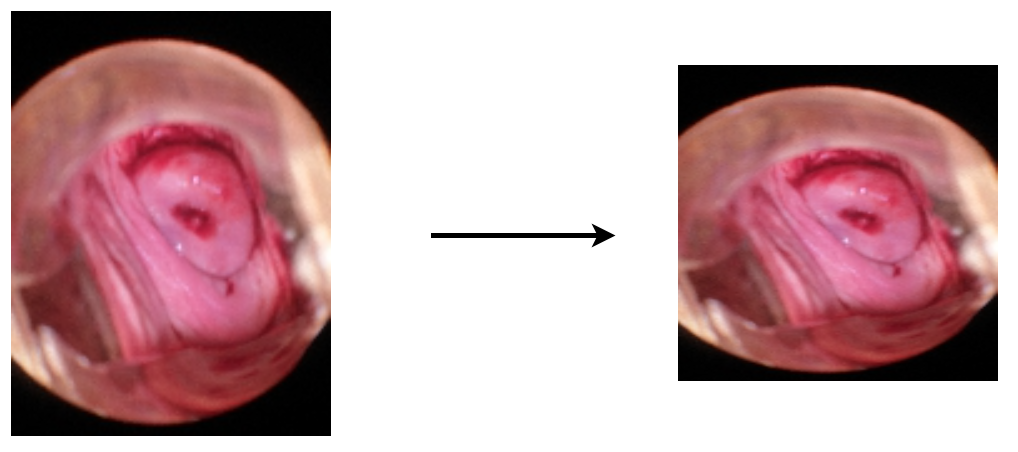
\includegraphics[scale=0.4]{./Capitulo2/imagenes/resize.png}
		\caption{Deformaci�n de la imagen al redimensionar.}
	\label{resize}
\end{figure} 

\section{Data Aumentation}
\label{aumentation}
Uno de los principales problemas en \textit{deep learning} es la falta de datos. Para ello, pueden usarse t�cnicas de \textit{data aumentation} que consisten en aplicar ligeras transformaciones a las im�genes para conseguir un conjunto de entrenamiento mayor, pudiendo obtener de una sola imagen 5 o 6 variaciones que enriquecen enormemente el modelo. Para ello, usando las funciones propias de Keras hemos aplicado las siguientes transformaciones a las im�genes:

\pagebreak
\clearpage
%---------------------------------------------------